% !TEX TS-program = xelatex
\documentclass[aspectratio=169]{beamer}

% --- THEME & LAYOUT ---
\usetheme[numbering=fraction,progressbar=head]{metropolis}
\setbeamersize{text margin left=8mm,text margin right=8mm}

% --- CUSTOM FOOTER WITH TLP MARKING ---
\setbeamertemplate{frame footer}{\textbf{TLP:CLEAR} – Information may be shared freely without restriction.}
\setbeamercolor{frame footer}{fg=cyber-accent}

\usepackage{amsmath}

% --- FONTS (XeLaTeX) ---
\usepackage{fontspec}
\setsansfont[
  Ligatures=TeX, Scale=1.02,
  BoldFont = {IBM Plex Sans Bold},
  ItalicFont = {IBM Plex Sans Italic}
]{IBM Plex Sans}
\setmonofont{IBM Plex Mono}

% --- ICONS ---
\usepackage{fontawesome5}

% --- COLORS (cyber palette) ---
\definecolor{cyber-bg}{HTML}{0B0F14}
\definecolor{cyber-ink}{HTML}{E6EEF5}
\definecolor{cyber-accent}{HTML}{217EAA}
\definecolor{cyber-mid}{HTML}{7D9CB7}
\definecolor{cyber-soft}{HTML}{8CA4AC}
\setbeamercolor{normal text}{fg=cyber-ink,bg=cyber-bg}
\setbeamercolor{frametitle}{fg=cyber-ink,bg=cyber-bg}
\setbeamercolor{progress bar}{fg=cyber-accent,bg=cyber-soft}
\setbeamercolor{alerted text}{fg=cyber-accent}

% --- LINKS ---
\hypersetup{colorlinks=true, linkcolor=cyber-accent, urlcolor=cyber-accent}

% --- CODE / BOXES ---
\usepackage{listings}
\lstset{
  basicstyle=\ttfamily\footnotesize,
  backgroundcolor=\color{black!5},
  frame=single, rulecolor=\color{cyber-soft},
  keywordstyle=\color{cyber-accent}\bfseries,
  commentstyle=\color{cyber-soft},
  showstringspaces=false
}
\usepackage[most]{tcolorbox}
\tcbset{colback=black!5!cyber-bg, colframe=cyber-soft, coltext=cyber-ink, boxsep=1mm, left=2mm, right=2mm}

% --- PDF TOOLS ---
\usepackage{pdfpages}

% --- GRAPHICS ---
\usepackage{graphicx}

% --- SPEAKER NOTES ---
\usepackage{pgfpages}
% \setbeameroption{hide notes}
% \setbeameroption{show notes}
% \setbeameroption{show only notes}

% --- SPACING IMPROVEMENTS ---
% Reduce spacing in itemize/enumerate globally for Beamer
\setbeamertemplate{itemize/enumerate body begin}{\vspace{-0.5ex}}
\setbeamertemplate{itemize/enumerate subbody begin}{\vspace{-0.5ex}}

% --- TITLE INFO ---
\title{\faIcon{shield-alt}\; Range42 Status Update}
\subtitle{Open Cyber Range Platform for Collaborative Security Training}
\author{NC3 / Range42 Team - Steve Clement}
\date{\today}
\institute{\faServer\; Proxmox \quad \faCogs\; Ansible \quad \faProjectDiagram\; Orchestration \quad \faBinoculars\; Telemetry}

\begin{document}

% --- TITLE ---
\begin{frame}[plain,noframenumbering]
  \titlepage
  \note[item]{Goal: 20-minute overview of Range42's progress and community collaboration opportunities.}
  \note[item]{Audience: open source contributors, cybersecurity educators, researchers.}
\end{frame}

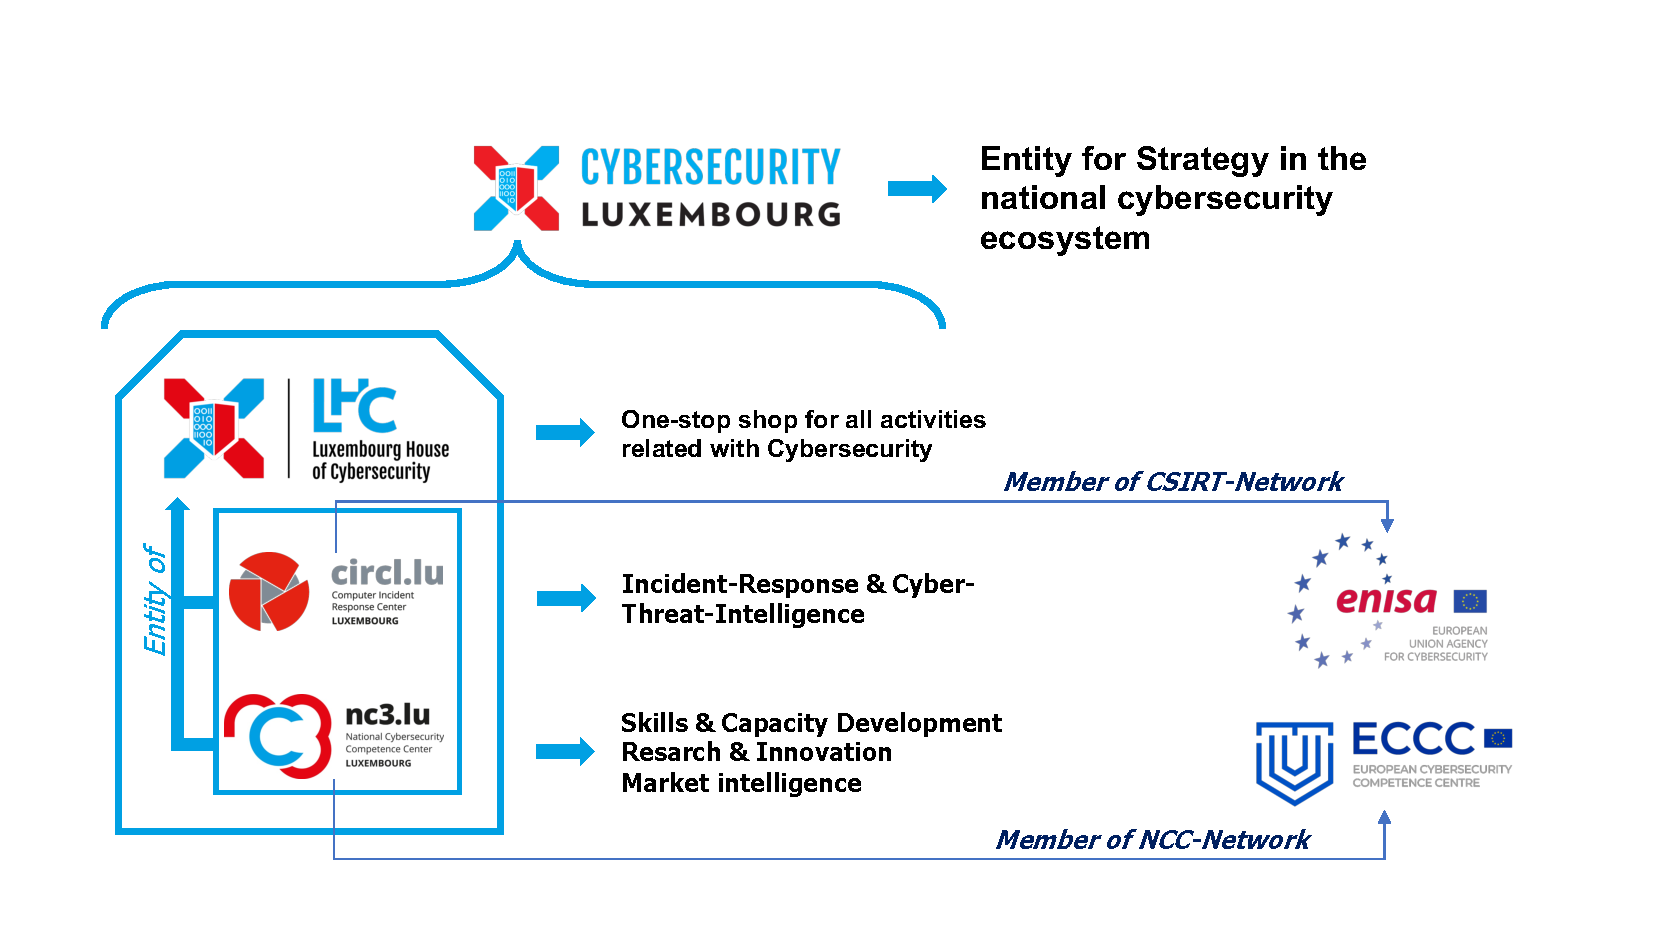
\includepdf[pages={1-2}]{pdf_slides/LHC_NC3.pdf}

% --- PUBLIC MONEY PUBLIC CODE ---
\begin{frame}[shrink=8]{Public money, public code. Let's go all the way, shall we?}
  \begin{columns}[T]
    \column{0.65\textwidth}
    \textbf{Current Team}
    \begin{itemize}
      \item Core development team of 3 contributors
      \item Mix of InfoSec \& DevOps engineers
      \item Collab model with NC3 \& ecosystem partners
    \end{itemize}
    
    \textbf{Current Funding}
    \begin{itemize}
      \item Public grant for cyber training infrastructure
      \item FOSS model: no licensing \textcolor{green}{\faMoneyBill}, transparent development
      \item Investment in reusable, community-driven tooling
    \end{itemize}
    
    \column{0.3\textwidth}
    \vspace{2mm}
    \begin{figure}
      \centering
      
\includegraphics[width=\textwidth]{images/logos/FSFE_Public_Money_Public_Code_logo.pdf}
    \end{figure}
  \end{columns}
  \note[item]{Emphasize public funding → public ownership → public benefit.}
\end{frame}

\begin{frame}[squeeze]{Public money, public code. Let's go all the way, shall we?}
  \begin{columns}[T]
    \column{0.65\textwidth}
    \textbf{Why We Need Your Help}
    \begin{itemize}
      \item Expanding scenario coverage requires diverse security expertise
      \item UI/UX design needs user-focused contributors
      \item Infrastructure automation benefits from community patterns
    \end{itemize}
    
    \textbf{Join Us}
    \begin{itemize}
      \item Open dev: all code, docs, and issues are public
      \item Welcoming to first-time contributors
      \item Apply to join the team $\xrightarrow{\hspace{4cm}}$
    \end{itemize}
    
    \column{0.3\textwidth}
    \vspace{10mm}
    \begin{figure}
      \centering
      
\includegraphics[width=\textwidth]{images/work-with-us-qrcode.png}
    \end{figure}
  \end{columns}
  \note[item]{Set collaborative tone early: this is a community project seeking contributors.}
\end{frame}

% --- AGENDA ---
\begin{frame}{Agenda}
  \begin{enumerate}
    \item What Range42 is \& why it matters
    \item Current achievements \& capabilities
    \item Architecture overview
    \item Development tracks: where we're heading
    \item How to contribute: scenarios, automation, UI/UX
    \item Lessons learned \& open challenges
  \end{enumerate}
  \note[item]{Keep flow brisk; emphasize collaboration opportunities throughout.}
\end{frame}

% --- WHAT IS RANGE42 ---
\begin{frame}{What is Range42?}
  \begin{itemize}
    \item \textbf{Open cyber range platform} for offensive, defensive, and hybrid training
    \item \textbf{Reproducible Infrastructure-as-Code}: Proxmox, Ansible, Docker
    \item \textbf{Flexible \& extensible}: supports CVE labs, misconfigurations, future malware/forensics scenarios
  \end{itemize}
  \begin{tcolorbox}
    \faInfoCircle\; Built to simulate \emph{real-world incidents} safely, with isolation, snapshots, and telemetry.
  \end{tcolorbox}
  \note[item]{Anchor on "safe realism" and extensibility for different training types.}
\end{frame}

% --- CURRENT ACHIEVEMENTS ---
\begin{frame}{Current Achievements \; \faCheckCircle}
  \textbf{What's Working Today}
  \begin{itemize}
    \item \alert{~100 CVEs \& misconfigurations identified} across common technologies
    %\item \alert{~20 scenarios currently deployable} for hands-on training
    \item \textbf{Automated provisioning} on Proxmox with networking, VPN, firewalling
    \item \textbf{Integrated monitoring} via Wazuh for telemetry and alerting
    \item \textbf{14 repositories} managing automation, content, and tooling
  \end{itemize}
  \vspace{2mm}
  \begin{tcolorbox}
    \faLightbulb\; \textbf{Key Milestone}: Platform is functional and actively used for internal testing training exercises.
  \end{tcolorbox}
  \note[item]{Emphasize concrete progress: this isn't vaporware, it's a working platform.}
  \note[item]{Highlight the gap: 100 identified but only 20 deployable = opportunity for contribution.}
\end{frame}

% --- COMPETITIVE LANDSCAPE ---
\begin{frame}[shrink=5]{Range42 vs. Other Cyber Ranges}
  \begin{table}
    \tiny\color{cyber-ink}
    \begin{tabular}{l|cccc}
      \textbf{Feature} & \textbf{Range42} & \textbf{Commercial SaaS} & \textbf{Cloud Native} & \textbf{Traditional} \\
      \hline
      \alert{Open Architecture} & \checkmark & \texttimes & \texttimes & \texttimes \\
      \alert{IaC/GitOps} & \checkmark & \textasciitilde & \checkmark & \texttimes \\
      Private Deployment & \checkmark & \texttimes & \textasciitilde & \checkmark \\
      Cost Control & \checkmark & \texttimes & \textasciitilde & \checkmark \\
      Full Data Custody & \checkmark & \texttimes & \texttimes & \checkmark \\
      API Orchestration & \checkmark & \checkmark & \checkmark & \texttimes \\
      Rapid Reset/Snapshots & \checkmark & \checkmark & \textasciitilde & \textasciitilde \\
      Custom Scenarios & \checkmark & \texttimes & \textasciitilde & \checkmark \\
    \end{tabular}
  \end{table}
  \vspace{1mm}
  \begin{tcolorbox}
    \faLightbulb\; \textbf{Range42's Edge}: Full control, reproducibility, and cost-effectiveness without vendor lock-in.
  \end{tcolorbox}
  \note[item]{Emphasize open architecture and IaC as key differentiators.}
  \note[item]{Commercial SaaS: SimSpace, Immersive Labs, RangeForce, Cyberbit.}
\end{frame}

% --- ARCH OVERVIEW ---
\begin{frame}[squeeze]{Architecture at a Glance}
  \begin{itemize}
    \item \textbf{Hypervisor layer}: Proxmox VMs/LXCs; snapshots; network segments
    \item \textbf{Automation layer}: Ansible roles orchestrate lifecycle, network, firewall, images
    \item \textbf{Control plane}: Backend API (routes for VM/Net/Runner); Kong gateway
    \item \textbf{UX}: Deployer UI (visual designer), EMP mockup (exercise management)
    \item \textbf{Observability}: Wazuh for logs/alerts; structured telemetry
  \end{itemize}
  \note[item]{Emphasize modularity: builder/deployer/runner + gateway.}
  \note[item]{Each layer is extensible and welcomes contributions.}
\end{frame}

\begin{frame}[shrink=8]{Architecture: Logical Components → Repository Mapping}
  \begin{figure}
    \centering
    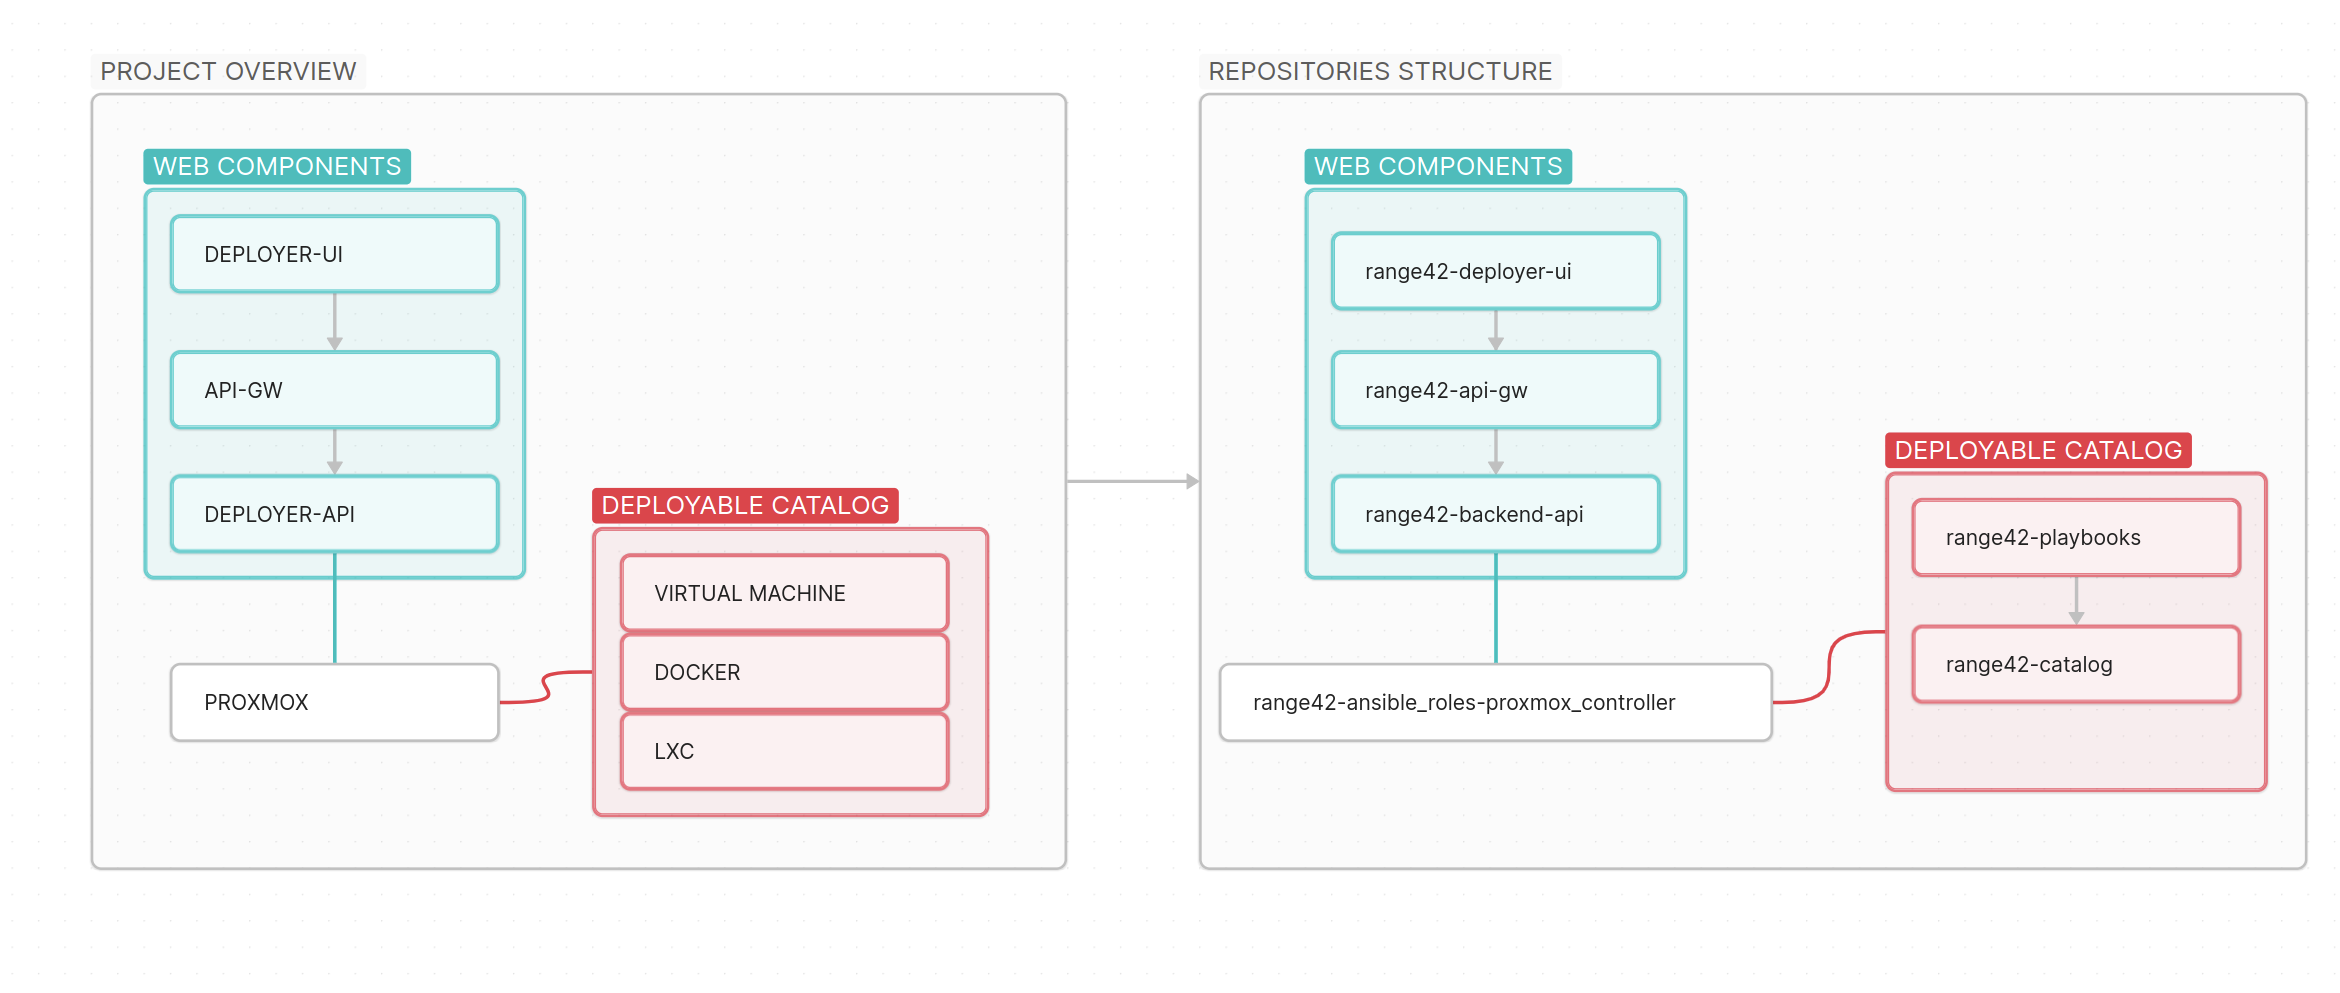
\includegraphics[width=0.95\textwidth]{images/diagrams/architecture.png}
  \end{figure}
  \vspace{-3mm}
  \begin{tcolorbox}
    \faInfoCircle\; \textbf{Left}: Logical architecture flow. \textbf{Right}: Actual GitHub repository structure.
  \end{tcolorbox}
  \note[item]{Left side shows logical architecture; right side shows actual GitHub repos.}
  \note[item]{Web components flow through API gateway to backend, which controls Proxmox via Ansible.}
  \note[item]{Deployable catalog (playbooks + catalog repos) contains the infrastructure-as-code content.}
\end{frame}

% === DEVELOPMENT TRACKS ===
\section{Development Tracks}

\begin{frame}[shrink=5]{Where We're Heading: Three Development Tracks \; \faRoad}
  \begin{enumerate}
    \item \textbf{Expand Vulnerability \& Misconfiguration Catalog}
    \begin{itemize}
      \item Goal: Increase from 20 to 50+ deployable scenarios
      \item Cover diverse technologies: web, network, cloud, containers
      \item Community contributions welcome for CVE research and deployment automation
    \end{itemize}
    
    \item \textbf{Advance Lab Designer from PoC to Production}
    \begin{itemize}
      \item Visual node-based infrastructure designer (VueFlow)
      \item Instructor-friendly: drag-and-drop scenario composition
      \item Export to Ansible playbooks for deployment
    \end{itemize}
    
    \item \textbf{Multi-Subnet Infrastructure Support}
    \begin{itemize}
      \item Simulate complex enterprise networks (DMZ, internal, management zones)
      \item Advanced firewall rules and traffic segmentation
      \item Support for red team / blue team exercises
    \end{itemize}
  \end{enumerate}
  \note[item]{These are the three tracks from the abstract - concrete, achievable goals.}
\end{frame}

% === KEY REPOSITORIES ===
\section{Key Repositories}

\begin{frame}[squeeze]{Organization Overview \; \faClipboardCheck}
  \textbf{14 Repositories Analyzed} (10 public, 4 private)\\[2mm]
  
  \textbf{Current State}
  \begin{itemize}
    \item \alert{Strong security baseline}: Zero high-severity findings across all code scans
    \item \alert{Governance standardization in progress}: LICENSE, SECURITY, CI/CD, contributor docs
    \item \alert{Active development}: 179 commits (devkit), 125 (backend), 108 (proxmox controller)
  \end{itemize}
  \vspace{1mm}
  \begin{tcolorbox}
    \faUsers\; \textbf{Contribution Opportunities}: Help us complete governance files, add CI pipelines, and expand scenario coverage.
  \end{tcolorbox}
  \note[item]{Frame governance gaps as opportunities for contribution, not problems.}
  \note[item]{Emphasize security is solid - we need help with structure and scale.}
\end{frame}

\begin{frame}[squeeze]{range42-ansible\_roles-proxmox\_controller \; \faCogs}
  \textbf{Status:} Active \hfill \textbf{Commits:} 108 \hfill \textbf{Lang:} Ansible/YAML\\[2mm]
  \textbf{Purpose:} Core automation for managing Proxmox nodes via API: VMs, LXC containers, networking, storage, firewall, and snapshots.\\[2mm]
  \textbf{Contribution Opportunities}
  \begin{itemize}
    \item Add CI pipeline with ansible-lint and Molecule idempotence tests
    \item Document role variables and provide example playbooks
    \item Extend functionality for advanced networking scenarios
  \end{itemize}
  \note[item]{Core infrastructure automation - heart of the platform.}
  \note[item]{Great entry point for Ansible contributors.}
\end{frame}

\begin{frame}[squeeze]{range42-backend-api \; \faProjectDiagram}
  \textbf{Status:} Active \hfill \textbf{Commits:} 125 \hfill \textbf{Lang:} Python/FastAPI\\[2mm]
  \textbf{Purpose:} FastAPI backend orchestrating Proxmox deployments via Ansible, with routes for VM control, networking, and bundle execution.\\[2mm]
  \textbf{Contribution Opportunities}
  \begin{itemize}
    \item Add unit tests and integration tests with pytest
    \item Improve error handling and validation
  \end{itemize}
  \note[item]{Well-structured backend with clean security scans.}
  \note[item]{Good target for Python/API developers.}
\end{frame}

\begin{frame}[squeeze]{range42-deployer-ui \; \faDrawPolygon}
  \textbf{Status:} Prototype \hfill \textbf{Commits:} 28 \hfill \textbf{Lang:} Vue/TypeScript\\[2mm]
  \textbf{Purpose:} VueFlow-based visual orchestrator for designing, validating, and deploying Range42 infrastructure through node-based interface.\\[2mm]
  \textbf{Contribution Opportunities}
  \begin{itemize}
    \item UI/UX improvements for instructor workflows
    \item Integration testing with backend API
    \item Export/import hardening for scenario sharing
  \end{itemize}
  \note[item]{This is the "lab designer" mentioned in development tracks.}
  \note[item]{Great opportunity for frontend/UX contributors.}
\end{frame}

\begin{frame}[squeeze]{range42-playbooks \& range42-catalog \; \faCubes}
  \textbf{Status:} Active \hfill \textbf{Commits:} 75 + 91 \hfill \textbf{Lang:} Ansible/YAML\\[2mm]
  \textbf{Purpose:} Centralized orchestration playbooks and reusable content catalog for deploying vulnerable scenarios and infrastructure bundles.\\[2mm]
  \textbf{Contribution Opportunities}
  \begin{itemize}
    \item \alert{Add new CVE scenarios}: research, document, automate deployment
    \item Introduce scenario taxonomy and tagging system
    \item Document compatibility matrices and dependencies
  \end{itemize}
  \note[item]{Content repositories - where the 100 CVEs live.}
  \note[item]{This is the highest-impact area for security researchers to contribute.}
\end{frame}

% === HOW TO CONTRIBUTE ===
\section{How to Contribute}

\begin{frame}[squeeze]{How to Contribute \; \faUsers}
  \textbf{Three Primary Contribution Paths}\\[2mm]
  
  \begin{columns}[T]
    \column{0.3\textwidth}
    \textbf{Scenario Design}
    \begin{itemize}
      \item CVE research
      \item Misconfig labs
      \item Documentation
    \end{itemize}
    
    \column{0.35\textwidth}
    \textbf{Infrastructure Automation}
    \begin{itemize}
      \item Ansible roles/playbooks
      \item Backend API features
      \item CI/CD pipelines
    \end{itemize}
    
    \column{0.3\textwidth}
    \textbf{UI/UX Design}
    \begin{itemize}
      \item Lab designer
      \item Exercise mgmt
      \item User workflows
    \end{itemize}
  \end{columns}
  \vspace{3mm}
  \begin{tcolorbox}
    \faGithub\; \textbf{Get Started}: Visit \texttt{github.com/range42} (public repos) or contact us for private repo access.
  \end{tcolorbox}
  \note[item]{Make contributing concrete: three clear paths with specific tasks.}
  \note[item]{Mention both public repos and process for private repo contributions.}
\end{frame}

\begin{frame}[squeeze]{Getting Started: Choose \& Setup}
  \textbf{Step 1: Choose Your Path}
  \begin{itemize}
    \item Browse open issues on GitHub (labeled "good first issue" and "help wanted")
    \item Review scenario inventory to find gaps in coverage
    \item Check documentation for areas needing clarity
  \end{itemize}
  
  \textbf{Step 2: Set Up Your Environment}
  \begin{itemize}
    \item Fork repositories and clone locally
    \item Follow setup guides in README files
    \item Join our communication channels (contact us for access)
  \end{itemize}
  \note[item]{First two steps: discovery and environment setup.}
\end{frame}

% commented out
\begin {comment}
\begin{frame}{Getting Started: Contribute \& Engage}
  \textbf{Step 3: Submit Your Contribution}
  \begin{itemize}
    \item Create pull request with clear description
    \item Ensure tests pass (where CI exists)
    \item Engage with code review feedback
  \end{itemize}
  
  \textbf{What to Expect}
  \begin{itemize}
    \item Friendly, constructive code reviews
    \item Response within 3-5 business days
    \item Recognition in contributors list and release notes
  \end{itemize}
  \note[item]{Final step plus expectations to encourage new contributors.}
\end{frame}
\end{comment}

% === LESSONS LEARNED ===
\section{Lessons Learned}

\begin{frame}[squeeze]{Lessons Learned \; \faLightbulb}
  \textbf{What We've Discovered}\\[2mm]
  
  \textbf{Technical Insights}
  \begin{itemize}
    \item \alert{Ansible + Proxmox API = powerful combo} for IaC cyber ranges
    \item Snapshot/restore capabilities are critical for training resets
    \item Telemetry integration from day one simplifies troubleshooting
  \end{itemize}
\end{frame}
  
\begin{frame}[squeeze]{Lessons Learned \; \faLightbulb}
  \textbf{Process \& Collaboration}
  \begin{itemize}
    \item \alert{Governance overhead is real}: LICENSE, SECURITY, CI/CD take time but unlock collaboration
    \item Documentation maturity lags code development (common open source challenge)
    %\item Balancing rapid prototyping with production-ready standards
  \end{itemize}
  \note[item]{Be honest about challenges - it builds trust with contributors.}
  \note[item]{Emphasize that these are normal open source growing pains.}
\end{frame}

% === OPEN CHALLENGES ===
\begin{frame}[shrink=5]{Open Challenges \& Opportunities \; \faExclamationTriangle}
  \textbf{Where We Need Help}\\[2mm]
  
  \textbf{Governance \& Quality}
  \begin{itemize}
    \item Enable CI/CD pipelines (ansible-lint, pytest, npm audit)
    \item Add contributor documentation and onboarding guides
  \end{itemize}
  
  \textbf{Technical Scaling}
  \begin{itemize}
    \item Expand scenario coverage from 20 to 50+ deployable labs
    \item Support multi-subnet architectures for complex exercises
  \end{itemize}
  \vspace{1mm}
  \begin{tcolorbox}
    \faUsers\; \textbf{Your Expertise Matters}: Every contribution - code, docs, testing, design - moves the platform forward.
  \end{tcolorbox}
  \note[item]{Frame challenges as opportunities for impactful contributions.}
\end{frame}

% === WRAP-UP ===
\begin{frame}[squeeze]{Range42: Today \& Tomorrow \; \faCheckCircle}
  \textbf{What We've Built}
  \begin{itemize}
    %\item Open, modular cyber range with ~20 deployable scenarios
    \item Open, modular cyber range
    \item Strong security baseline: zero high-severity findings
    \item Clear architecture with multiple contribution paths
    \item Active development: 13 repositories, 500+ commits
  \end{itemize}
  \vspace{2mm}
  \textbf{What We're Building}
  \begin{itemize}
    \item 50+ scenario coverage across diverse technologies
    \item Production-ready lab designer for instructors
    \item Multi-subnet support for advanced training exercises
  \end{itemize}
  \note[item]{Summary slide: current state and future direction.}
\end{frame}

\begin{frame}[shrink=10]{Get Involved \; \faRocket}
  \begin{columns}[T]
    \column{0.65\textwidth}
    \textbf{Join the Range42 Community}\\[1mm]
    
    \textbf{Contribution Areas}
    \begin{itemize}
      \item \textbf{Scenario Design}: CVE research, automation
      \item \textbf{Infrastructure}: Ansible roles, backend API, CI/CD
      \item \textbf{UI/UX}: Lab designer, EMP UI
    \end{itemize}
    \vspace{1mm}
    \textbf{Contact \& Resources}
    \begin{itemize}
      \item Web: \texttt{range42.lu}
      \item GitHub: \texttt{github.com/range42}
      \item Email: \texttt{steve.clement@nc3.lu}
    \end{itemize}

   \vspace{2\baselineskip}
    \noindent \textcolor{white}{Typeset with \LaTeX{}} {\textcolor{blue}{\faHeart}}

    
    \column{0.3\textwidth}
    \vspace{0mm}
    \begin{figure}
      \centering
      
\includegraphics[width=\textwidth]{images/contribute.png}
      \caption*{\footnotesize \textcolor{white}{github.com/range42}}
    \end{figure}
  \end{columns}
  \note[item]{Final call to action with clear next steps and contact information.}
\end{frame}

\end{document}